%************************************************
\chapter{Experimental Setup}
\label{chp:experimental_setup}
%************************************************



\iffalse
Chicago 1m, evaluera denna * 
Chicago 7m, evaluera denna *
Sampla mindre 1m och 7m (3 av varje, totalt 4 med original) (10s, 20s, 50s) - run times
Chicago 7m 0 *
Chicago 7m 1 *
Chicago 7m 2 * 

OSM 2012 *
OSM 2012 1m verifierad *
OSM 2012 7m verifierad *
(OSM 2018)
OSM slingan (ta ut motorvägar/använda mapfuse)

Athen small 
- kolla sampling
- kolla yta
- syfte: lägga ihop flera små rutor

DriveMe
- kör genom eval, jämför med osm
- skriv om problematik med lane level (metod + lane level = False, använd annan metod!)


Max dist in map fuse
samplingsfrekvens
mängd data som används för att skapa en karta
 - antal gps punkter per total väglängd

\fi

% \textbf{något om att vi tog fram experiment som var av intresse för zenuity... utgick från det när vi gjorde vår experimental setup}

The experiments are run in Python 3 on an MacBook Pro (13-inch, 2017, Four Thunderbolt 3 Ports) with a 3,1 GHz Intel Core i5 processor running Mac OS Sierra 10.13.3.

We designed experiments that were of interest to Zenuity. For example we demonstrate how the algorithms scale with time and the area covered by trajectories. In particular, much effort was put into how to evaluate the maps when they have been created. Both inferred maps will be compared to one another, but also they will be compared to the ``ground truth'' being our ``verified'' \ac{OSM}. 

% The experiments are run in Matlab on an Intel Xeon W3500 PC with 4GB RAM running Windows 7.

%========================================================================%
\section{OSM}
%========================================================================%
\label{chp:experimental_setup.sec:osm}
 
In table \ref{tab:osm_exp_setup} we present all \ac{OSM} used throughout the experiments. We have previously mentioned that \cite{biagioni:gis12} made their code public which can be found at \citep{chicago}. Here, they had also uploaded an \ac{OSM} from 2012 which they used in their evaluations. This will be referred to as COSM12 and contained all roads in the area of interest, meaning more roads then had been traversed by the bus. We also chose to use COSM12 as a base when ``verifying'' two maps, COSM12\_1m and COSM12\_7m, according to the description in section \ref{chp:data.sec:osm.sec:gt}. Furthermore, we downloaded the present \ac{OSM} (from 2018), COSM18, to compare the current \ac{OSM} to the one from 2012. \textbf{gothenburgh and athens...}


\begin{table}[H]
\centering
\caption{Information about \ac{OSM} that was used in the experiments. The column verified indicates if we have verified the map according to the, if stated, given data set.}
\label{tab:osm_exp_setup}
\begin{tabular}{cccc}
location   & year & verified         & map name            \\ \hline
Chicago    & 2012 & no               & COSM12              \\
Chicago    & 2012 & 1 month          & COSM12\_1m \\ % $_{ver, 1m}$ \\
Chicago    & 2012 & 7 month          & COSM12\_7m \\ %$_{ver, 7m}$\\
Chicago    & 2018 & no               & COSM18              \\ \hline
%Gothenburg & 2018 & no               & GOSM                \\
%Athen      & \textbf{missing}     & no               & AOSM                \\ \hline
\end{tabular}
\end{table}


%========================================================================%
\section{Map generation}
%========================================================================%
\label{chp:experimental_setup.sec:mapgen}

To test the performance of the map generation we varied the amount of data and size of the area of interest used to create a map. Two aspects will be taken into account---time scalability and evaluation scores. 

The inferred maps were created according to the pipeline described in section \ref{chp:method.sec:map} using data sets described in section \ref{chp:data.sec:gpsdata}. In table \ref{tab:mapgen_exp_setup:chicago_maps} a summary of all created inferred maps using the Chicago data sets is displayed. The first two, C1m and C7m, are created using the Chicago 1 month data set and the Chicago 7 month data set. The rest are explained in more detail in the following sections. In table \ref{tab:mapgen_exp_setup:other_maps} the inferred maps created using other data sets are displayed. \textbf{gothenburgh and athens...}

\begin{table}[H]
\centering
\caption{Maps created from Chicago data sets.}
\label{tab:mapgen_exp_setup:chicago_maps}
\begin{tabular}{cccc}
data set        & sampling rate & region & map name                \\ \hline
Chicago 1 month & n.a.        & n.a.   & C1m                     \\
Chicago 7 month & n.a.        & n.a.   & C7m                     \\
Chicago 1 month & 10          & n.a.   & C1m$_{10}$ \\ 
Chicago 1 month & 20          & n.a.   & C1m$_{20}$ \\ 
Chicago 1 month & 50          & n.a.   & C1m$_{50}$ \\
Chicago 7 month & n.a.        & 0      & C7m$_0$  \\
Chicago 7 month & n.a.        & 1      & C7m$_1$  \\
Chicago 7 month & n.a.        & 2      & C7m$_2$  \\ \hline
\end{tabular}
\end{table}

\begin{table}[H]
\centering
\caption{Maps created from DriveMe and Athens data sets.}
\label{tab:mapgen_exp_setup:other_maps}
\begin{tabular}{cc}
data set & map name     \\ \hline
DriveMe  & DM           \\
Athens   & A            \\ \hline
\end{tabular}
\end{table}


%------------------------------------------------------------------------%
\subsection{Less frequently sampled data}
%------------------------------------------------------------------------%

Since storing a lot of data requires a lot of storage, it is of great interest to understand how little data we can use to still get a map that represents the road network with sufficient accuracy. Therefore experiments were performed using less frequently sampled data. Looping thorough all trajectories, a sample (a \ac{GPS} point), was removed if less then 10, 20 and 50 seconds had passed since the previous one. 

Three data sets with sampling rates 10, 20 and 50 seconds were created this way using the Chicago 1 month data set, see section \ref{chp:data.sec:gpsdata.sec:chicago}. Then corresponding maps C1m$_{10}$, C1m$_{20}$ and C1m$_{50}$ were created using the pipeline described in section \ref{chp:method}. The trajectories in each data set cover an area of 3.92421×2.39023 km$^2$, 3.92421×2.38468 km$^2$, 3.92421×2.3668 km$^2$ respectively. Further information of the three new data sets are displayed in tables \ref{tab:C1m_10_exp_setup}, \ref{tab:C1m_20_exp_setup}, \ref{tab:C1m_50_exp_setup} and \ref{tab:exp_setup_102050_bbox}.

% 10 s
\begin{table}[H]
\centering
\caption{Specifications for Chicago 1 month 10 second sampling rate data set.}
\label{tab:C1m_10_exp_setup}
\begin{tabular}{cccccc}
      & \# traces & \# samples & \begin{tabular}[c]{@{}c@{}}sampling\\ rate {[}s{]}\end{tabular} & length {[}km{]} & \begin{tabular}[c]{@{}c@{}}duration\\ {[}d hh:mm:ss{]}\end{tabular} \\ \hline
total & 889.00    & 30'904.00  & n.a.                                                        & 2'815.68 & 4 21:07:05                                                      \\
min   & n.a.      & 13.00      & 11.00                                                       & 2.21     & 00:02:20                                                        \\
max   & n.a.      & 90.00      & 39.00                                                       & 8.65     & 00:20:12                                                        \\
mean  & n.a.      & 34.76      & 14.05                                                       & 3.17     & 00:07:54                                                        \\
std   & n.a.      & 9.74       & 4.83                                                        & 0.88       & 00:02:18                                                        \\ \hline
\end{tabular}
\end{table}

% 20 s
\begin{table}[H]
\centering
\caption{Specifications for Chicago 1 month 20 second sampling rate data set.}
\label{tab:C1m_20_exp_setup}
\begin{tabular}{cccccc}
      & \# traces & \# samples & \begin{tabular}[c]{@{}c@{}}sampling\\ rate {[}s{]}\end{tabular} & length {[}km{]} & \begin{tabular}[c]{@{}c@{}}duration\\ {[}d hh:mm:ss{]}\end{tabular} \\ \hline
total & 889.00    & 18'131.00  & n.a.                                                        & 2'737.70 & 4 19:48:44                                                      \\
min   & n.a.      & 8.00       & 21.00                                                       & 2.07     & 00:02:30                                                        \\
max   & n.a.      & 51.00      & 49.00                                                       & 8.45     & 00:20:04                                                        \\
mean  & n.a.      & 20.39      & 24.18                                                       & 3.08     & 00:07:49                                                        \\
std   & n.a.      & 5.69       & 4.90                                                        & 0.87       & 00:02:18                                                        \\ \hline
\end{tabular}
\end{table}

% 50 s
\begin{table}[H]
\centering
\caption{Specifications for Chicago 1 month 50 second sampling rate data set.}
\label{tab:C1m_50_exp_setup}
\begin{tabular}{cccccc}
      & \# traces & \# samples & \begin{tabular}[c]{@{}c@{}}sampling\\ rate {[}s{]}\end{tabular} & length {[}km{]} & \begin{tabular}[c]{@{}c@{}}duration\\ {[}d hh:mm:ss{]}\end{tabular} \\ \hline
total & 889.00    & 8'379.00   & n.a.                                                        & 2'497.75 & 4 16:26:17                                                      \\
min   & n.a.      & 3.00       & 51.00                                                       & 1.67     & 00:01:43                                                        \\
max   & n.a.      & 24.00      & 79.00                                                       & 8.14     & 00:20:19                                                        \\
mean  & n.a.      & 9.43       & 54.04                                                       & 2.81     & 00:07:35                                                        \\
std   & n.a.      & 2.57       & 4.77                                                        & 0.84       & 00:02:19                                                        \\ \hline
\end{tabular}
\end{table}

% bbox
\begin{table}[H]
\centering
\caption{Bounding boxes for each data set.}
\label{tab:exp_setup_102050_bbox}
\begin{tabular}{ccccc}
                                 &     & \begin{tabular}[c]{@{}c@{}}Chicago 1m\\ 10 s\end{tabular} & \begin{tabular}[c]{@{}c@{}}Chicago 1m\\ 20 s\end{tabular} & \begin{tabular}[c]{@{}c@{}}Chicago 1m\\ 50 s\end{tabular} \\ \hline
\multirow{2}{*}{latitude [decimal °]}        & min & 41.862                                                    & 41.862                                                    & 41.862                                                    \\
                                 & max & 41.884                                                    & 41.884                                                    & 41.883                                                    \\
\multirow{2}{*}{longitude [decimal °]}       & min & -87.687                                                   & -87.687                                                   & -87.687                                                   \\
                                 & max & -87.640                                                   & -87.640                                                   & -87.640                                                   \\
area [km$^2$] &     & 9.380                                                     & 9.358                                                     & 9.288                                                     \\ \hline
\end{tabular}
\end{table}

%------------------------------------------------------------------------%
\subsection{Three regions}
%------------------------------------------------------------------------%

To further evaluate fusing maps we divided up the Chicago 7 month data set in three data sets according to region. It was divided up into three geographic regions; 0, 1 and 2. To illustrate this, figure \ref{fig:exp_setup/regions} and table \ref{tab:exp_setup:regions} were included. Each ``number region'' in table \ref{tab:exp_setup:regions} consisted of all \ac{GPS} points in the corresponding ``letter regions'' displayed in figure \ref{fig:exp_setup/regions}. Every trip file was looped thorough from beginning to end. If and when a trip file started in one region and continued into another the trip was divided up into the same number of new trip files. More information about the new trip files and data sets can be found in tables \ref{tab:C7m_0_exp_setup}, \ref{tab:C7m_1_exp_setup} and \ref{tab:C7m_2_exp_setup}.

For the regions 0, 1 and 2 corresponding maps C7m$_0$, C7m$_1$ and C7m$_2$ were created using the pipeline described in section \ref{chp:method}. The area of interest is displayed in table \ref{tab:exp_setup_012_bbox}. The trajectories in each region data set cover an area of 3.89×2.46 km$^2$, 1.94616×2.31348 km$^2$ and 1.94624×2.451 km$^2$ respectively.

\begin{table}[H]
\centering
\caption{Explanation of going from letter regions in figure \ref{fig:exp_setup/regions} to number regions, making up the three data sets.}
\label{tab:exp_setup:regions}
\begin{tabular}{cc}
Region number & Region letter \\ \hline
0             & a, b          \\
1             & b, c          \\
2             & c, d          \\ \hline
\end{tabular}
\end{table}

% regions
\begin{figure}[H]
    \centering
    \includegraphics[width=12cm]{Figures/Experimental_Setup/regions.pdf}
    \caption{Illustration how the Chicago 7 month data set was divided up according to region.}
    \label{fig:exp_setup/regions}
\end{figure}

% 0
\begin{table}[H]
\centering
\caption{Specifications for Chicago 7 month region 0 data set.}
\label{tab:C7m_0_exp_setup}
\begin{tabular}{cccccc}
      & \# traces & \# samples & \begin{tabular}[c]{@{}c@{}}sampling\\ rate {[}s{]}\end{tabular} & length {[}km{]} & \begin{tabular}[c]{@{}c@{}}duration\\ {[}d hh:mm:ss{]}\end{tabular} \\ \hline
total & 4'094.00  & 574'609.00 & n.a.                                                        & 13'851.80   & 32 13:58:24                                                     \\
min   & n.a.      & 3.00       & 1.00                                                        & 0.05        & 00:00:04                                                        \\
max   & n.a.      & 257.00     & 598.00                                                      & 6.46        & 00:37:50                                                        \\
mean  & n.a.      & 140.35     & 4.93                                                        & 3.38        & 00:11:28                                                        \\
std   & n.a.      & 45.57      & 13.14                                                       & 1.13        & 00:03:22                                                        \\ \hline
\end{tabular}
\end{table}

% 1
\begin{table}[H]
\centering
\caption{Specifications for Chicago 7 month region 1 data set.}
\label{tab:C7m_1_exp_setup}
\begin{tabular}{cccccc}
      & \# traces & \# samples & \begin{tabular}[c]{@{}c@{}}sampling\\ rate {[}s{]}\end{tabular} & length {[}km{]} & \begin{tabular}[c]{@{}c@{}}duration\\ {[}d hh:mm:ss{]}\end{tabular} \\ \hline
total & 8'621.00  & 917'000.00 & n.a.                                                        & 22'378.41   & 45 22:18:35                                                     \\
min   & n.a.      & 2.00       & 1.00                                                        & 0.02        & 00:00:02                                                        \\
max   & n.a.      & 273.00     & 598.00                                                      & 6.52        & 00:45:25                                                        \\
mean  & n.a.      & 106.37     & 4.37                                                        & 2.60        & 00:07:40                                                        \\
std   & n.a.      & 46.41      & 11.12                                                       & 1.15        & 00:04:29                                                        \\ \hline
\end{tabular}
\end{table}

% 2
\begin{table}[H]
\centering
\caption{Specifications for Chicago 7 month region 2 data set.}
\label{tab:C7m_2_exp_setup}
\begin{tabular}{cccccc}
      & \# traces & \# samples & \begin{tabular}[c]{@{}c@{}}sampling\\ rate {[}s{]}\end{tabular} & length {[}km{]} & \begin{tabular}[c]{@{}c@{}}duration\\ {[}d hh:mm:ss{]}\end{tabular} \\ \hline
total & 4'097.00  & 679'507.00 & n.a.                                                        & 16'612.33   & 43 13:24:49                                                     \\
min   & n.a.      & 2.00       & 1.00                                                        & 0.02        & 00:00:02                                                        \\
max   & n.a.      & 861.00     & 599.00                                                      & 20.55       & 01:39:46                                                        \\
mean  & n.a.      & 165.85     & 5.57                                                        & 4.05        & 00:15:19                                                        \\
std   & n.a.      & 77.54      & 20.24                                                       & 1.86        & 00:08:20                                                        \\ \hline
\end{tabular}
\end{table}

% bbox
\begin{table}[H]
\centering
\caption{Bounding boxes for each data set.}
\label{tab:exp_setup_012_bbox}
\begin{tabular}{ccccc}
                                           &     & \begin{tabular}[c]{@{}c@{}}Chicago 1m\\ region 0\end{tabular} & \begin{tabular}[c]{@{}c@{}}Chicago 1m\\ region 1\end{tabular} & \begin{tabular}[c]{@{}c@{}}Chicago 1m\\ region 2\end{tabular} \\ \hline
\multirow{2}{*}{latitude {[}decimal °{]}}  & min & 41.866                                                        & 41.862                                                        & 41.862                                                        \\
                                           & max & -87.687                                                       & 41.883                                                        & 41.884                                                        \\
\multirow{2}{*}{longitude {[}decimal °{]}} & min & 41.883                                                        & -87.675                                                       & -87.663                                                       \\
                                           & max & -87.663                                                       & -87.652                                                       & -87.640                                                       \\
area [km$^2$]           &     & 3.566                                                         & 4.502                                                         & 4.770                                                         \\ \hline
\end{tabular}
\end{table}



\subsection{Athens and DriveMe}

\textbf{gothenburgh and athens...}


\subsection{Summary of map generation experiments}

% Run times will be reported on map generation of the divided 7 month Chicago data set in region 0, 1 and 2 with corresponding maps;

We chose to first evaluate the generated maps, both using other inferred maps but also using our verified \ac{OSM}. A summary of this is found in table \ref{tab:evalinfmaps}. The base map is used as ground truth to evaluate the new map. Furthermore, we evaluate the \ac{OSM} from 2012 and compare it with the \ac{OSM} from 2018 to see if we can detect changes that has occurred since then. The maps will be evaluated using three different evaluation metrics presented in section \ref{chp:method.sec:evaluation}.

\begin{table}[H]
\centering
\caption{Summary of map generation experiments.}
\label{tab:evalinfmaps}
\begin{tabular}{ccc}
\begin{tabular}[c]{@{}c@{}}map generation\\ experiment\end{tabular} & base map   & new map \\ \hline
MG1                                                                 & COSM12\_1m & C1m     \\
MG2                                                                 & COSM12\_7m & C7m     \\
MG3                                                                 & C1m        & C7m     \\
MG4                                                                 & C7m        & C1m     \\ 
MG5                                                                 & COSM12     & COSM18  \\ \hline
\end{tabular}
\end{table}

Furthermore, time scalability was investigated using the inferred maps. The less frequently sampled data sets were used to experiment with how much data is needed to create a sufficiently accurate map. 


%========================================================================%
\section{Map fuse}
%========================================================================%

Using the generated maps in table \ref{tab:mapgen_exp_setup:chicago_maps} we will now perform experiments where some of these will be fused using the method described in section \ref{chp:method.sec:fuse}. A summary of all the experiments is displayed in table \ref{tab:mapfuse_exp_setup}. Here we will test how well the map fuse 


\begin{table}[H]
\centering
\caption{Map fuse tests using inferred maps created from the Chicago data sets.}
\label{tab:mapfuse_exp_setup}
\begin{tabular}{ccccc}
\begin{tabular}[c]{@{}c@{}}map fuse\\ experiment\end{tabular} & base map     & new map  & fused map                     & test             \\ \hline
MF1 & C1m          & C7m      & C$_{\text{1m},\text{7m}}$     & delete/add edges \\
MF2 & C7m          & C1m      & C$_{\text{7m},\text{1m}}$     & delete/add edges \\
MF3 & C7m$_0$      & C7m$_1$  & C$_{\text{7m}_{0,1}}$                   & add edges        \\
MF4 & C7m$_2$      & C7m$_1$  & C$_{\text{7m}_{2,1}}$                   & add edges        \\
MF5 & C7m$_{0,1}$  & C7m$_2$  & C$_{\text{7m}_{(0,1),2}}$               & add edges        \\ 
MF6 & COSM12\_1m          & COSM12\_7m      & COSM\_12$_{\text{1m},\text{7m}}$     & add edges \\
MF7 & COSM12\_7m          & COSM12\_1m      & COSM\_12$_{\text{7m},\text{1m}}$     & add edges \\
MF8 & COSM12      & COSM18  & COSM$_{12,18}$                   & add edges        \\ 
MF9 & COSM12\_1m & C7m & COSM\_12\_1m$_{\text{7m}}$ & add edges \\
MF10 & COSM12\_7m & C1m & COSM\_12\_7m$_{\text{1m}}$ & add edges \\
\hline
\end{tabular}
\end{table}


%------------------------------------------------------------------------%
\subsection{Decision making}
%------------------------------------------------------------------------%
Three types of changes between maps will be investigated

\begin{itemize}
    \item new roads
    \item temporary changes
    \item old roads to be removed.
\end{itemize}

The tests performed for the decision making procedure for each type of change is explained in more detail in the following sections.

%........................................................................%
\subsubsection{Add roads}
\label{chp:experiments.sec:mapfuse.sub:dec.sub:add}
%........................................................................%
The map fusion method described in section \ref{chp:method.sec:fuse} has parameters that needs to be tuned. The thresholds are
\begin{itemize}
    \item densify distance
    \item bearing difference
    \item matching distance
    \item outlier distance.
\end{itemize}
The smaller the densify distance is the more accurate the fusion will be.   

The optimal values for each parameter is further dependent on the quality of the maps to be fused. 

%........................................................................%
\subsubsection{Delete roads}
%........................................................................%



parametertuning...





%------------------------------------------------------------------------%
\subsection{Two suggested routines}
%------------------------------------------------------------------------%

We propose two methodologies for creation and updating of maps. The first uses the \ac{OSM} as a base map and new roads from the inferred map will be added to the existing \ac{OSM}. The second one will instead be consisting of inferred roads only. A routine was created for checking which roads exist in the \ac{OSM} and which ids could be confirmed.

%........................................................................%
\subsubsection{OSM as base map}
%........................................................................%

Remove some roads in the OSM...

%........................................................................%
\subsubsection{Inferred maps exclusively}
%........................................................................%


\paragraph{Comparing to OSM}


%========================================================================%
\section{Parameter tuning}
\label{ch:experiments.sec:paramtuning}
%========================================================================%

Among the set based evaluation methods both the geometric (GEO) and the topological (TOPO) evaluation described in sections \ref{chp:method.sec:evaluation.sub:geom} and \ref{chp:method.sec:evaluation.sub:topo} respectively have parameters that needs to be tuned. These were chosen such that the quality of the evaluation was estimated to be high enough and the run time was kept as low as possible. The GEO method has the following parameter:
\begin{itemize}
    \item sample spacing.
\end{itemize}
That is the spacing in meters between each sample on edges in the maps. The TOPO evaluation has the following:
\begin{itemize}
    \item sample spacing 
    \item maximum path length from start location
    \item number of local samples.
\end{itemize}
These parameters were varied as presented in table \ref{tab:experiments/paramtune}. The data set used for the evaluation presented here was the Chicago 1 month data set. The chosen values were shown to give similar results also for the other data sets.

\begin{table}[H]
\centering
\caption{The tests performed for parameter tuning of set based evaluation methods.}
\label{tab:experiments/paramtune}
\begin{tabular}{cc}
parameter & test \\ \hline
sample spacing & 1-50 m \\
max sampling distance & 100-1000 m \\
\# evaluations & 10-500 \\ \hline
\end{tabular}
\end{table}

%%%% SAMPLE DENSITY %%%%%
In figure \ref{fig:experiments/marker_dens} we plot the result of GEO when varying the sample spacing. The result was seen to be equivalent when the spacing was below about 10 meters. Considering also that the run times, presented in table \ref{tab:experiments/marker_dens}, increased as the spacing was made too low the sample spacing was fixed to 5 meters.
\begin{figure}[H]
    \centering
    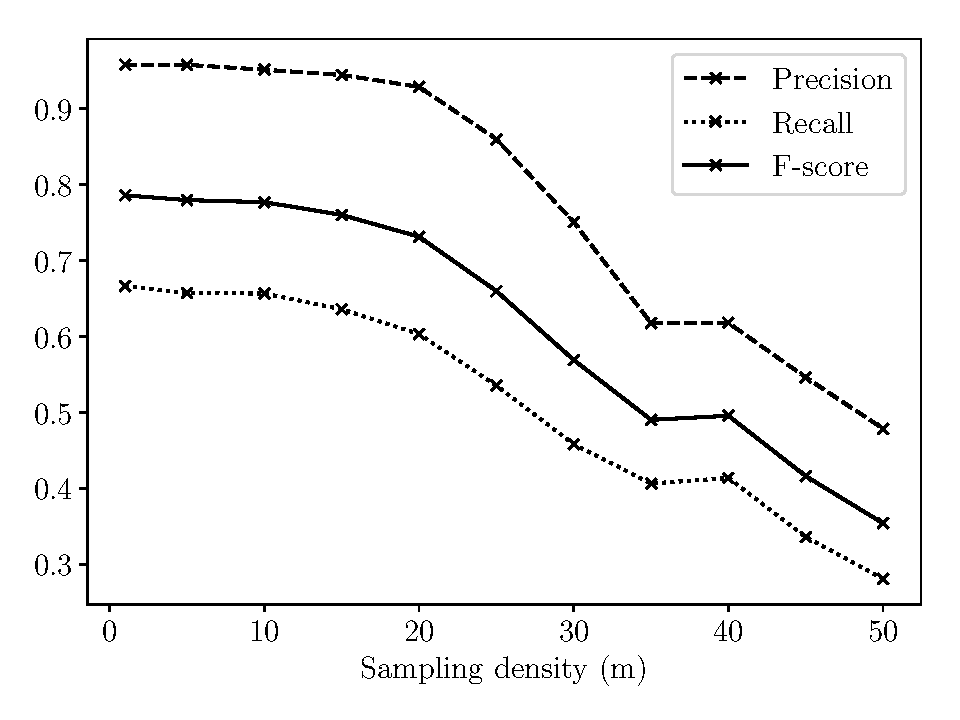
\includegraphics[width=9cm]{Figures/Experimental_Setup/test_marker_density.pdf}
    \caption{GEO evaluation of Chicago 1 month data set. The sample spacing along edges in the maps was varied from 1 to 50 meters.}
    \label{fig:experiments/marker_dens}
\end{figure}

\begin{table}[H]
\centering
\caption{Run times for the GEO evaluation of Chicago 1 month data set with different sample spacings.}
\label{tab:experiments/marker_dens}
\begin{tabular}{cc}
sample spacing (m) & time (s) \\ \hline
1 & 8.77 \\
5 & 0.64 \\
10 & 0.25 \\ 
30 & 0.07 \\
\hline
\end{tabular}
\end{table}

%%%% MAX SAMPLE DIST %%%%%
In figure \ref{fig:experiments/samp_dist} the result of the TOPO evaluation when varying the maximum sampling distance from the start location can be seen. The sample spacing was fixed at 5 m and the number of evaluations at 100. This distance should be large enough for us to capture the similarity of the neighbourhood of each starting point, for example at intersections. The mean distance between intersections in the maps was calculated to be about 350 meters. As the distance increases the run time for the evaluation increases significantly, which is demonstrated in table \ref{tab:experiments/samp_dist}. A reasonable value was concluded to be about 300 meters.

\begin{figure}[H]
    \centering
    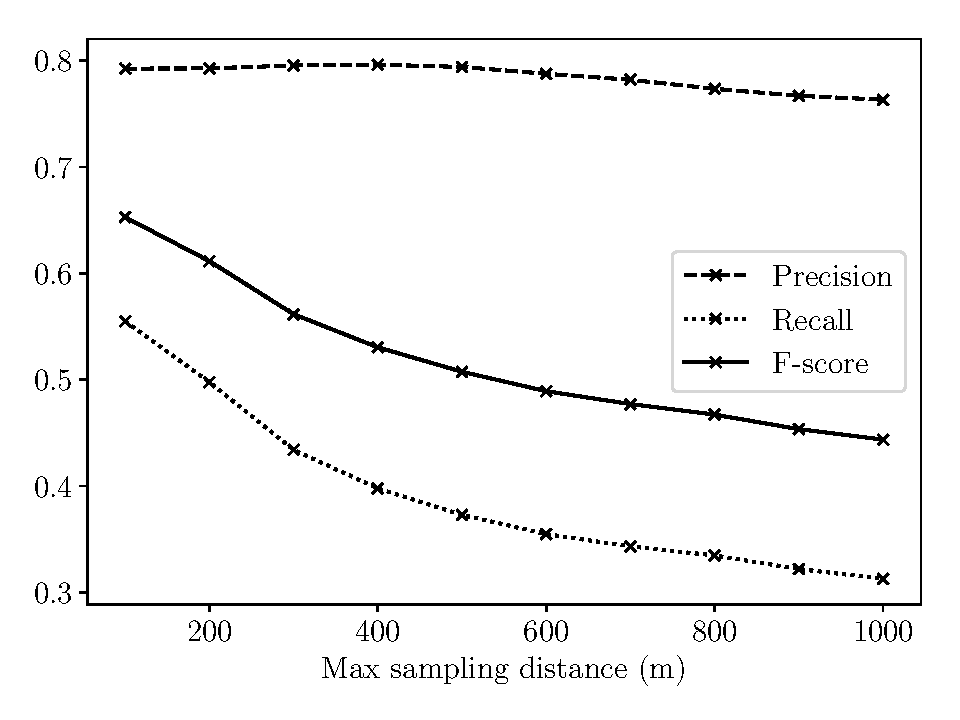
\includegraphics[width=9cm]{Figures/Experimental_Setup/test_sample_dist.pdf}
    \caption{TOPO evaluation of Chicago 1 month data set. The max sampling distance was varied from 100 to 1000 meters.}
    \label{fig:experiments/samp_dist}
\end{figure}

\begin{table}[H]
\centering
\caption{Run times for the TOPO evaluation of Chicago 1 month data set with different max sampling distance.}
\label{tab:experiments/samp_dist}
\begin{tabular}{cc}
sampling distance (m) & time (s) \\ \hline
100 & 2.54 \\
300 & 8.10 \\
500 & 32.24 \\
1000 & 113.76 \\ \hline
\end{tabular}
\end{table}

%%%% NUM EVALS %%%%%
In figure \ref{fig:experiments/num_evals} we plot the result of the TOPO evaluation when varying the number of evaluations for each run. The sample spacing was fixed at 5 m and the max sampling distance at 300 m. The result was seen to be equivalent after around 150 evaluations. This value was thus fixed to 150.
\begin{figure}[H]
    \centering
    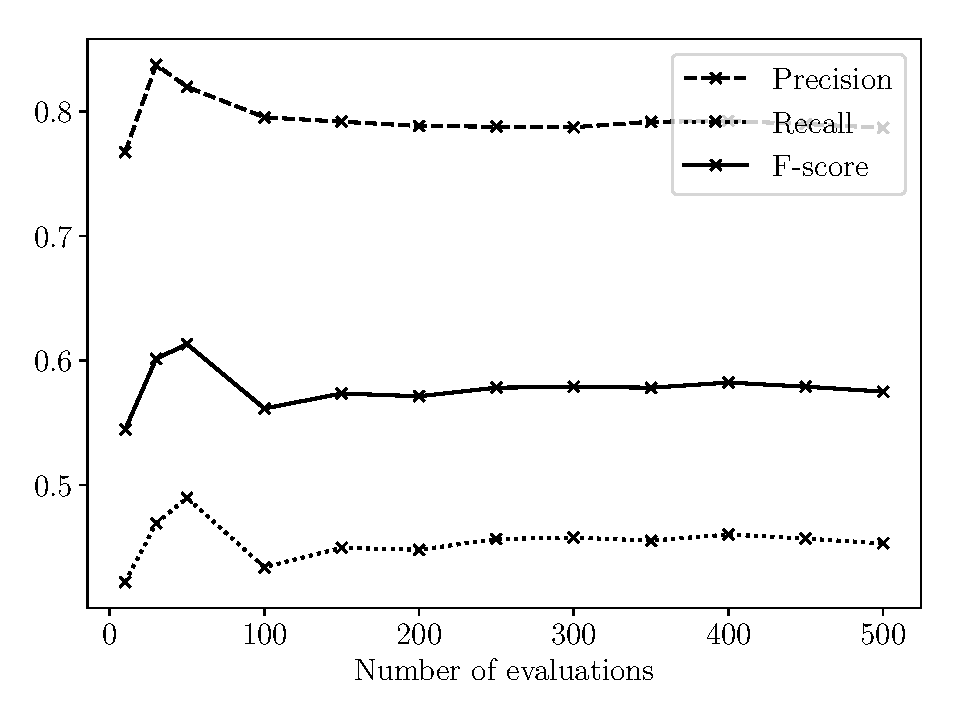
\includegraphics[width=9cm]{Figures/Experimental_Setup/test_num_evals.pdf}
    \caption{TOPO evaluation of Chicago 1 month data set. The number of evaluations was varied from 10 to 500.}
    \label{fig:experiments/num_evals}
\end{figure}

\begin{table}[H]
\centering
\caption{Run times for the TOPO evaluation of Chicago 1 month data set with different number of evaluation runs.}
\label{tab:experiments/num_evals}
\begin{tabular}{cc}
\# evaluations & time (s) \\ \hline
10 & 0.72 \\
100 & 6.99 \\
300 & 21.37 \\
500 & 35.81 \\ \hline
\end{tabular}
\end{table}

A summary of the parameter tuning is reported below.

\begin{table}[H]
\centering
\caption{A summary of the results of parameter tuning for the set based map comparison methods.}
\label{tab:experimenst/tuning}
\begin{tabular}{cc}
parameter & value \\ \hline
sample spacing & 5 m \\
max sample distance & 300 m \\
\# evaluations & 150 \\ \hline
\end{tabular}
\end{table}


%========================================================================%
\section{Lane level}
%========================================================================%


